% !TeX document-id = {117ac6b5-8dd4-4613-9231-0768b5815107}
%pdflatex -shell-escape exos.tex
%pythontex exos.tex
%pdflatex -shell-escape exos.tex
% !TeX TXS-program:compile = txs:///pdflatex/[--shell-escape]

\documentclass[12pt,french]{article}
\usepackage[utf8]{inputenc}
\usepackage{array,multicol,multirow,enumerate,eurosym,latexsym,fourier,bbding,pifont}
\usepackage{fourier}
\usepackage{graphicx,pst-all}
\usepackage{tabularx}
\usepackage [alwaysadjust]{paralist}
\usepackage{amsmath,amsfonts,amsthm,amssymb,geometry}
\usepackage{fancyhdr}
\usepackage{mathrsfs}  
%\usepackage{table}
\usepackage{pstricks,pst-plot,pst-text,pst-tree,pstricks-add,pst-eps,pst-fill,pst-node,pst-math}
\usepackage{euscript,amsfonts,eepic,color}
\usepackage{ifthen,fp}
\newcommand{\Calig}[1]{\ensuremath{\mathscr{#1}}}              
\usepackage{babel}
\usepackage{xcolor}
\usepackage{minted}
\usepackage{pythontex}
\usepackage{multicol}
\usepackage[most]{tcolorbox}
\usepackage{fancyhdr}
\setlength{\parindent}{0pt}
\usepackage{ulem}
\usepackage[np]{numprint}
\geometry{vmargin=15mm,hmargin=5mm}
\pagestyle{empty}
\setlength\columnsep{5mm}
\renewcommand{\thesection}{\Roman{section}}
\renewcommand{\thesubsection}{\Alph{subsection}}
\renewcommand{\thesubsubsection}{\arabic{subsubsection}}
\newcounter{npb}
\setcounter{npb}{0}
\newcommand{\exo}{
    \stepcounter{npb}
    {\textbf{$\triangleright$ \underline{Exercice \arabic{npb} }}}
}
\newcounter{sf}
\setcounter{sf}{0}
\newcommand{\s}{
    \stepcounter{sf}
    {\textbf{ \fbox{SF \arabic{sf} }}}
}
\usepackage{lscape}
\usepackage{tikz}
\usepackage{metalogo}
\usepackage{hyperref}
\begin{document}

  \lhead{Lycée Jean Monnet - \textit{NSI}}
    \chead{}
    \rhead{\textit{Année} 2019/2020}
      \renewcommand{\headrulewidth}{0.5pt}
      \lfoot{                      }\cfoot{Page \thepage}\rfoot{\textsf{Aude Duhem et Patrice Nicolas}}
    \pagestyle{fancy}
    \renewcommand{\footrulewidth}{0.4pt}
\begin{center}
\textbf{\Large{Les algorithmes gloutons - Feuille d'exercices   }}\end{center}
\hrule
\bigskip
\exo  - Exercice débranché - $\star$ \\
On suppose dans cet exercice, qu'on prend le système de pièces de monnaie européen (en centimes)
\begin{enumerate}
	\item On suppose qu'on dispose d'autant d'unités que l'on veut.  Quel est le rendu de monnaie proposé à l'aide d'un algorithme glouton de monnaie 
	\begin{enumerate}
		\item si on doit rendre 2\euro 47 ?
		\item si on doit rendre 6\euro 36 ?
		\item si on doit rendre 3 \euro 68 ?
	\end{enumerate}
\item On suppose à présent qu'on a un nombre limité de pièces réparti de la façon suivante :\\
\begin{tabular}{|c|c|c|c|c|c|c|c|c|}
	\hline
	Pièces en centimes&200&100&50&20&10&5&2&1\\
	\hline
	Quantité&3&5&9&8&6&5&4&1\\
	\hline
	\end{tabular}\\
 Quel est le rendu de monnaie proposé à l'aide d'un algorithme glouton de monnaie si on doit rendre successivement 2\euro 47, 6\euro 36 et 3\euro 68 ? 

\end{enumerate}
\hrule
\medskip
\exo - Exercice débranché - $\star$ \\
On considère un bureau de poste américain qui ne dispose pas de machine à affranchir mais des timbres de valeurs faciales :\\
1 cent, 10 cents, 21 cents, 34 cents, 70 cents et 100 cents\\
Un client veut affranchir un courrier pour 1\$ et 40 cents.
\begin{enumerate}
	\item Quel serait le rendu proposé à l'aide d'un l'algorithme glouton de rendu de monnaie ? 
	\item A-t-on obtenu une solution optimale ? 
\end{enumerate}
\hrule
\medskip
\exo - Exercice débranché - $\star$ 
\begin{center}
\og Ils sont fous ces Bretons ! \fg
\end{center}
\begin{flushright}
Obélix dans Astérix chez les Bretons, Goscinny et Uderzo\\
\href{https://omnilogie.fr/O/Livre,\_shilling,\_penny...\_le\_syst\%C3\%A8me\_mon\%C3\%A9taire\_anglais\_avant\_la\_d\%C3\%A9cimalisation}{(Source)}
\end{flushright}
Nous sommes en 1966 après Jésus-Christ. Toutes les monnaies européennes sont décimalisées… Toutes ? Non ! Un royaume peuplé d'irréductibles Bretons résiste encore et toujours à la décimalisation de leur chère livre sterling. En effet, jusqu'en 1971, le Royaume-Uni ne possédait pas un système de monnaies décimalisées\footnote{Décimalisée signifie ici que la livre sterling est divisée en cent sous-unités : cent pence (au singulier : un penny). Un penny vaut un centième de livre.}. \\
La livre(\pounds) valait 20 shillings(s) et un shilling 12 pence(d). Il y avait d'autres sous-unités du penny et du shilling :\\
voici le récapitulatif des "petits" billets et des pièces qui étaient utilisés en 1966.
\footnotesize
\begin{center}
\begin{tabular}{|c|c|c|c|c|c|c|c|c|c|c|}
	\hline
	&\multicolumn{2}{c}{billets}&\multicolumn{8}{|c|}{Pièces}\\
	\hline
	Nom&a Fiver&a Quid&a Half-Crown&a Florin&a Bob&a Tanner&three Pence&a Copper&a half-penny&a farthing\\
	\hline
Valeur&5 \pounds&1 \pounds&2 shillings &two &one&six Pence&$\cfrac 1 4 $ shilling&one Penny&$\cfrac 1 2$ de penny&$\cfrac 1 4$ de penny\\
&&& and 6 pence&Shillings& Shilling&&&&&\\
\hline
Valeur&&&&&&&&&&\\
 en pence&&&&&&&&&&\\
\hline
\end{tabular}
\end{center}
\normalsize
\begin{enumerate}
	\item Compléter les dernières lignes du tableau.
	\item On se propose de tester un algorithme glouton de rendu de monnaie en prenant pour répartition de monnaie toutes les unités en pence décrites ci-dessus. On considère que l'on dispose d'autant d'unités que l'on veut.
		\begin{enumerate} 
		\item On doit rendre 2 \pounds\, et 34 pences. Quel serait le rendu proposé par l'algorithme ?
		
		\item On doit rendre 3 \pounds\, et 4 shillings. Quel serait le rendu proposé par l'algorithme ?
		\item A-t-on obtenu des solutions optimales ?
		\end{enumerate}
  
\end{enumerate} 
%https://omnilogie.fr/O/Livre,_shilling,_penny..._le_syst%C3%A8me_mon%C3%A9taire_anglais_avant_la_d%C3%A9cimalisation 
%https://fr.wikipedia.org/wiki/Livre_sterling#Guin%C3%A9e
\hrule
\medskip
\exo  - Exercice branché - $\star\star$ \\
Une route comporte $n$ stations-service, numérotées dans l'ordre du parcours, de 0 à $n-1$. Les distances entre chaque stations-service sont données par un tableau de données $d$ $[d_0,d_1, ...; d_n]$ telle que : \\
la première est à une distance $d_0$ du départ, la deuxième est à une distance $d_1$ de la première, la troisième à une distance $d_2$ de la deuxième, etc. La fin de la route est à une distance $d_n$ de la $n$-ième et dernière station-service.\\
Un automobiliste prend le départ de la route avec une voiture dont le réservoir d'essence est plein.
Sa voiture est capable de parcourir une distance r avec un plein.
\begin{enumerate}
\item Donner une condition nécessaire et suffisante pour que l'automobiliste puisse effectuer le
parcours. On la supposera réalisée par la suite.
\item En considérant 17 stations-service avec les distances d = [23, 40, 12, 44, 21, 9, 67, 32, 51, 30, 11, 55, 24,
64, 32, 57, 12, 80] et r = 100.\\
L'automobiliste désire faire le plein le moins souvent possible. Écrire une fonction en Python nommée rapide de paramètre $d$ et $r$ qui détermine à quelles stations-service il doit s'arrêter.
\end{enumerate}
\hrule

\medskip
\exo  - Exercice débranché - $\star$ \\
Le problème dit "du sac à dos" possède une importance majeure en algorithmique. Depuis plus d'un siècle, il fait l'objet de recherches actives et sa résolution trouve de nombreuses applications pratiques dans le domaine de la finance par exemple. Dans les années 1970, il fut a l'origine des premiers algorithmes de cryptographie à clé publique/privée. Nous tenterons de le résoudre par différentes "méthodes" gloutonnes.\\
\vspace{3mm}
\begin{tcolorbox}[enhanced,attach boxed title to top center={yshift=-3mm,yshifttext=-1mm},
	colback=red!5!white,colframe=red!75!black,colbacktitle=red!25!black,
	title=Enoncé du problème, fonttitle=\bfseries,
	boxed title style={size=small,colframe=red!25!black} ]
	\textbf{"Imaginons un voleur entrant de nuit dans un magasin ; il est équipé  d'un sac pour réaliser son délit et y placer les objets volés. Malheureusement pour lui, son sac est usé et au-delà d'un certain poids, celui-ci risque de craquer. Dès lors, pour maximiser son profit, le voleur cherche à placer dans son sac les objets de plus grande valeur possible, tout en veillant à ne pas dépasser le poids maximal autorisé."}
\end{tcolorbox}
\vspace{2mm}
\begin{enumerate}
	\item S'agit-il d'un problème d'optimisation ? Justifier la réponse.
	\begin{tcolorbox}[enhanced,attach boxed title to top center={yshift=-3mm,yshifttext=-1mm},
		colback=red!5!white,colframe=red!75!black,colbacktitle=red!25!black,
		title=Notations, fonttitle=\bfseries,
		boxed title style={size=small,colframe=red!25!black} ]
		On parle souvent du \textbf{KP} pour évoquer le problème du sac à dos  \textbf{(KP = "Knapsack Problem")}.\\
		On parle parfois du \textbf{0/1-KP} car les objets sont volés en entier (1) ou laissés dans le magasin (0) : le voleur ne peut pas prendre un bout d'objet ! Supposons que  quatre objets(A, B, C, et D) présents dans le magasin, et que le voleur vole les quatre : la solution du  \textbf{0/1-KP} peut-être notée \{1, 1, 1, 1\}
	\end{tcolorbox}
\item En utilisant les notations précédentes, quelle est la solution si le voleur vole les objets A et C ?
\item Soient trois objets de 4kg, 2kg et 1kg ainsi qu'un sac supportant jusqu'à 6kg. La solution \{1, 0, 1\} respecte-t-elle la condition sur la masse totale autorisée?

\end{enumerate} 
\newpage

\medskip
\exo  - Exercice débranché - $\star$ \\
Prenons l'exemple d'un sac supportant 4 kg au maximum et un magasin avec trois objets  A, B, C(Voir Figure 1). On supposera que le sac est suffisamment grand pour accueillir tous les objets.
Pour la suite nous représenterons, les trois objets sous la forme d'un couple  \textbf{(valeur en €, poids en kg):}
\begin{center}   Objet A:  (100, 2)\hspace{1cm} Objet B:  (10,2)\hspace{1cm}  Objet C: (120,3).\end{center}
\begin{figure}[h]
	\centering
	\caption{\label{overflow}}
	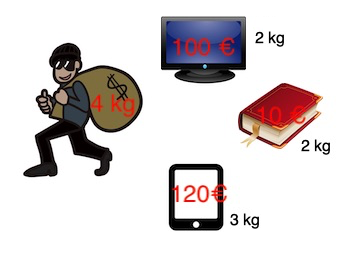
\includegraphics[width=90mm]{Sac}
	
\end{figure}
\begin{enumerate}
	
	\item En respectant le poids maximal, déterminer ("sur papier") le nombre de façons de remplir le sac (on pourra présenter les résultats dans un tableau). 
\item Indiquer quel est le choix le plus profitable au voleur.


\end{enumerate}
\hrule
\medskip
\exo Exercice débranché - $\star$  mais accès à la documentation officielle Python3\\
Soit la liste d'objets suivante où chaque objet est caractérisé par (un poids, une valeur) et un sac tel que $p_{max}=2,7$:\newline
L=[(0.2,300),(0.2,500),(0.1,250),(0.3,500),(1.3,2300),(0.8,2000),(1.3,2500)]
\vspace{2mm}
\begin{enumerate}
	\item Ecrire une liste triée par valeurs (décroissante) puis une liste triée par rapport décroissant $\frac{\text{valeur}}{\text{poids}}$

	
	
	\item Appliquer l'algorithme glouton sur ces deux listes et écrire une liste réponse uniquement constituée de 0 ou de 1. Commenter.

	\item En Python, que renvoie les instructions \mintinline{python}{L.sort(key = lambda a : a[1])}\\
	 et \mintinline{python}{L.sort(key = lambda a : a[0], reverse=True)} ?

\end{enumerate}	
\hrule
\medskip
\exo - exercice branché - $\star\star$  \\	
Il s'agit d'exécuter un algorithme "naïf" qui consiste à tester toutes les choix d'objets acceptables pour finir par choisir la meilleure. 
\begin{enumerate}
	\item Télécharger sur l'ENT le fichier \textbf{ex8.py}.
	\item Le code télechargé comporte plusieurs fonctions. La fonction \textbf{possibilites} de paramètre un entier $n$ permet d'afficher le nombre de choix possibles de $n$ objets (dans le sac du voleur).\\	Tester la fonction  \textbf{possibilites} pour   \(n \in \{3,4,5,6,7\} \). Conjecturer le nombre de façons de remplir le sac avec $n$ objets.
	\item La fonction \textbf{KPnaif} de paramètre une liste de couples  \textbf{(valeur en €, poids en kg)} et un entier $n$  retourne  un triplet constitué de la solution optimale obtenue par l'algorithme naïf pour le sac, la valeur du sac et le poids du sac. Tester l'algorithme et noter les durées d'exécution sur les 5 premiers jeux de données du fichier datas.txt, c'est à dire pour $n  \in \{4,7,8,10,15 \}$.
	\item  A l'aide du logiciel de votre choix, représenter $t=f(n)$ où $t$ représente la durée d'exécution du programme.\\
	 Donner une équation d'une courbe de tendance de la forme $t=a\times e^{b\times n}$ (donner les valeurs des paramètres a, b).
	\item Quel est le temps d'exécution prédit par ce modèle lorsque $n$ =50 ? Commenter le résultat obtenu.
\end{enumerate}	

\end{document}








